% !
\section{Area Between Curves}
In Calculus 2, the area between two curves refers to the region enclosed by two 
functions and the x-axis on a coordinate plane. The area between the curves can 
be found by subtracting the area under one function (the "bottom" function) from 
the area under the other function (the "top" function).\\

One way to find the area between the curves is by using definite integrals. The 
definite integral of a function gives the signed area under the curve of that 
function. The definite integral of a function over an interval [a, b] gives the 
signed area between the curve of that function and the x-axis over that 
interval. To find the area between two curves, we can find the definite integral 
of each function over the same interval, and then subtract the definite integral 
of the "bottom" function from the definite integral of the "top" function.\\

For example, if we have two functions f(x) and g(x), and we want to find the 
area between the curves for the interval [a, b], we can use the following 
formula: Area = $\int_{a}^{b}$ [f(x) - g(x)] dx\\

It is important to keep in mind that the definite integral gives the signed 
area, so if the "top" function is below the "bottom" function over the interval, 
the area between the curves will be negative.\\

Another way to find the area between the curves is by using Riemann Sums, which 
is a method that approximates the area between the curves by dividing the 
interval into smaller subintervals, and computing the area of rectangles with 
heights at the points of the function at the right endpoint of each 
subinterval.\\

It is important to note that when finding the area between curves, it is 
important to check the function and make sure that the area we are trying to 
find is the area between the curves and not the area of one of the functions.\\

In some cases, the area between the curves might not be continuous, in those 
cases we will have to split the region into smaller regions and find the area 
for each of them separately.\\

\begin{framed}
  \begin{align*}
    \text{Area} &= \int_{left}^{right} (\text{top} - \text{bottom}) \, dx\\\\
    \text{Area} &= \int_{bottom}^{top} (\text{right} - \text{left}) \, dy
  \end{align*}
\end{framed}

\newpage

\begin{framed}
  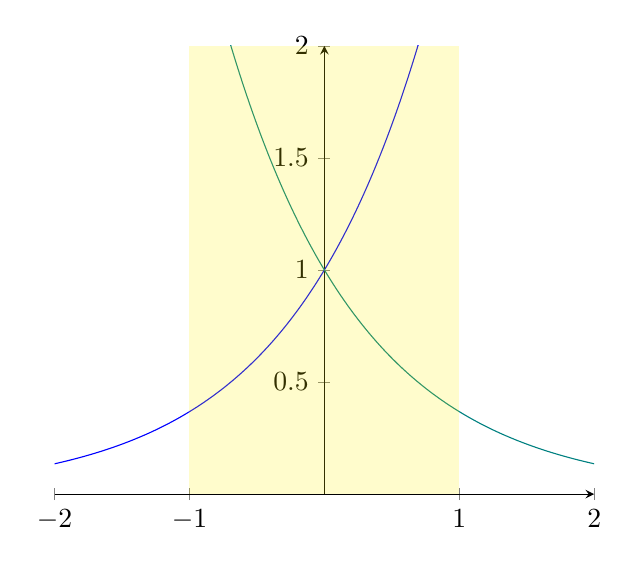
\begin{tikzpicture}
    \begin{axis}[axis x line=center, axis y line=center, xmin=-2, xmax=2, ymin=0, ymax=2, samples=100]
      \addplot[color=blue, smooth, domain=-2:2] {exp(x)};
      \addplot[color=teal, smooth, domain=-2:2] {exp(-x)};
      \drawplot[domain=.1:3] (\x, {ln(\x)});
      \fill[yellow, opacity=0.2] (axis cs:-1, 0) rectangle (axis cs:1, 2);
    \end{axis}
  \end{tikzpicture}
\end{framed}